\documentclass[12pt,a4paper]{article}
\usepackage[utf8]{inputenc}%Para Tildes y ñ%
\usepackage[spanish]{babel}
\usepackage{amsmath}
\usepackage{amsfonts}
\usepackage{amssymb}
\usepackage{siunitx}
\usepackage{adjustbox}
%\usepackage{minted}
\usepackage{listings}
\lstset{
  language=C,
  basicstyle=\ttfamily,
  keywordstyle=\color{red},
  stringstyle=\color{orange},
  commentstyle=\color{blue},
  numbers=left,
  numberstyle=\tiny\color{gray},
  stepnumber=1,
  frame=single,
  breaklines=true,
  breakatwhitespace=false,
  tabsize=2,
  captionpos=d
  inputencoding=utf8/latin1,
  keepspaces=true,
  showstringspaces=false,
  literate=%
    {á}{{\'a}}1
    {é}{{\'e}}1
    {í}{{\'i}}1
    {ó}{{\'o}}1
    {ú}{{\'u}}1
    {Á}{{\'A}}1
    {É}{{\'E}}1
    {Í}{{\'I}}1
    {Ó}{{\'O}}1
    {Ú}{{\'U}}1
    {ñ}{{\~n}}1
    {Ñ}{{\~N}}1
}

\usepackage[american]{circuitikz}
\usepackage{tikz}
\usepackage{graphicx} 
\usepackage{pdfpages} %para importar paginas de un pdf 
\usepackage{booktabs}
\usepackage{multicol}
\usepackage[bookmarks = true, colorlinks=true, linkcolor = black, citecolor = green, menucolor = black, urlcolor = black]{hyperref} 
\usepackage[left=2cm,right=2cm,top=2cm,bottom=2cm]{geometry} 
\usepackage{multirow}
\addto\captionsspanish{\renewcommand{\listtablename}{Índice de tablas}}		% Cambiar nombre a lista de tablas   
\addto\captionsspanish{\renewcommand{\tablename}{Tabla}}					% Cambiar nombre a tablas
\usepackage{float}		% Para ubicar las tablas y figuras justo después del texto
\usepackage{pdfpages}
\usepackage{enumerate}%listas y viñetas
\author{Estudiantes:\\ Kevin Campos Castro\\ Josué Salmerón Córdoba  \\{\small Grupo 1}\\ Profesor:  Marco Villalta  \vspace*{3.0in}}
\title{Universidad de Costa Rica\\{\small Facultad de Ingeniería\\Escuela de Ingeniería Eléctrica\\IE0624 – Laboratorio 5\\III ciclo 2023\\\vspace*{0.55in}}\\ STM32/Arduino: GPIO, Giroscopio, comunicaciones, TinyML. \vspace*{1.35in}}
%\date{fecha de entrega} 

\begin{document} 

\maketitle  
\thispagestyle{empty}%%no numerar la portada
\renewcommand{\thepage}{\roman{page}}
\newpage
\tableofcontents
\newpage
\listoffigures 
\newpage
\listoftables  
\newpage
%%%%%%%%%%  
\renewcommand{\thepage}{\arabic{page}} 
\setcounter{page}{1}
\begin{center}
\section{Resumen}
\end{center}
En este trabajo se presenta una de muchas aplicaciones en TinyML que posee el microcontrolador Arduino Nano 33 Ble Sense, en este caso se trata de la detección de movimientos realizados con el brazo. Con ayuda del ejemplo de la librería de TensorFlowLite, en especial el \texttt{IMU\_Capture} se logró hacer uso del giroscopio y la acelaración de los movimientos para luego hacer un entrenamiento de los datos con el notebook de Colab disponible en \cite{web4} y con el ejemplo \texttt{IMU\_Classifier} la placa logra identificar mostrando la probabilidad más alta de alguno de los 3 movimientos realizados. Por tanto, este trabajo cumple satisfactoriamente con lo solicitado porque el arduino es capaz de identificar los movimientos una vez realizados.
% AQUI VA EL RESUMEN 

%\textbf{\textit{Palabras clave}} \\

%palabras,clave,separadas, por,coma (solo en el reporte)
   
\newpage  


%\section{Objetivos}
\subsection{Objetivos General}
\begin{itemize}
\item obj gral. 

\end{itemize}

\subsection{Objetivos Específicos}
\begin{itemize}
\item objetivo 1
\item objetivo 2  

\end{itemize} 
\newpage
\section{Nota teórica}
En esta sección se describen los componentes principales que se utilizaron para el desarrollo del HAR-Human Activity Recognition.
\subsection*{ Arduino Nano 33 BLE}
El arduino Nano 33 BLE Sense es un módulo miniatura que contiene un módulo NINA B306, basado en Nordic nRF52480 y contiene un M4F Cortex, un cripto chip el cual puede almacenar certficados de forma segura y pre-compartir llaves y un IMU de 9 ejes. El módulo puede ser montado como un componente DIP o como componente SMT, directamente soldado por la via de los pads.
\subsubsection*{Características generales}
Las características más importantes de este mcu se mencionan a continuación \cite{web}
\begin{multicols}{2}
 \begin{itemize}
    \item CPU: ARM Cortex-M4 a 64MHz con FPU, 32-bit, 1MB Flash, 256kB SRAM.
    \item Bluetooth 5, IEEE 802.15.4-2006, \SI{2.4}{\giga\Hz}.
    \item ARM TrusZone Cryptocell 310 security subsystem, secure boot.
    \item USB 2.0, QSPI, SPI.
    \item 48 GPIOs.
    \item 12-bit, ADC con 8 canales.
    \item 64 comparadores de nivel, 15 del tipo low-power.
    \item Sensor de temperatura.
    \item $4\times4$-canales PWM.
    \item Periféricos de audio: I2S, PDM
    \item $5\times32$-bit timers.
    \item $4\times$ SPI maestros\/$3\times$ SPI esclavos.
    \item $2\times$I2C.
    \item $2\times$ UART.
    \item decodificador de cuadratura (QDEC).
    \item $3\times$ RTC.
\end{itemize}   
\end{multicols}
\newpage
\subsubsection*{Diagrama de bloques}
La figura \ref{fig1} representa el diagrama de bloques de la placa.
\begin{figure}[H]
\centering
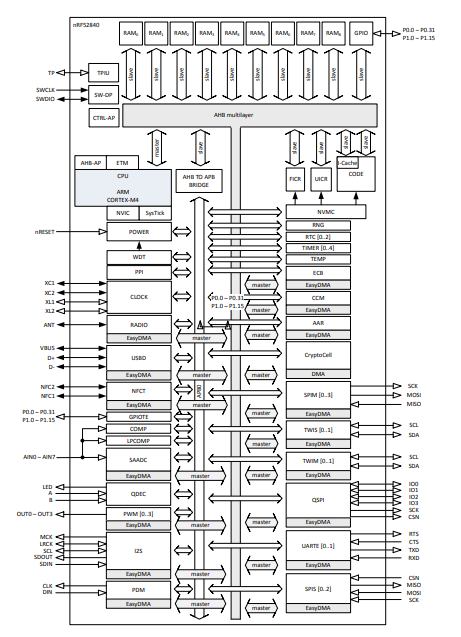
\includegraphics[width=.55\linewidth]{Imagenes/1.png}
 \caption{Diagrama de bloques del Nano BLE 33 Sense . Tomado de \cite{web}.}
 \label{fig1}
\end{figure}
\newpage
\subsubsection*{Diagrama de pines}
El diagrama de la fugura \ref{fig2} brinda de manera más detallada la distribución de los pines.
\begin{figure}[H]
\centering
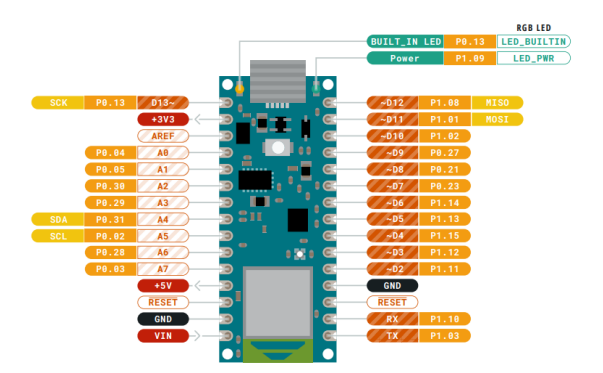
\includegraphics[width=.55\linewidth]{Imagenes/2.png}
 \caption{Diagrama de pines del Nano BLE 33 Sense . Tomado de \cite{web2}.}
 \label{fig2}
\end{figure}
\subsubsection*{Características eléctricas}
Aquí se tomaron dos referencias para tener más claro este detalle,  primero se muestran los valores máximos del mcu nRF52480 y los de la placa respectivamente.
\begin{figure}[H]
\centering
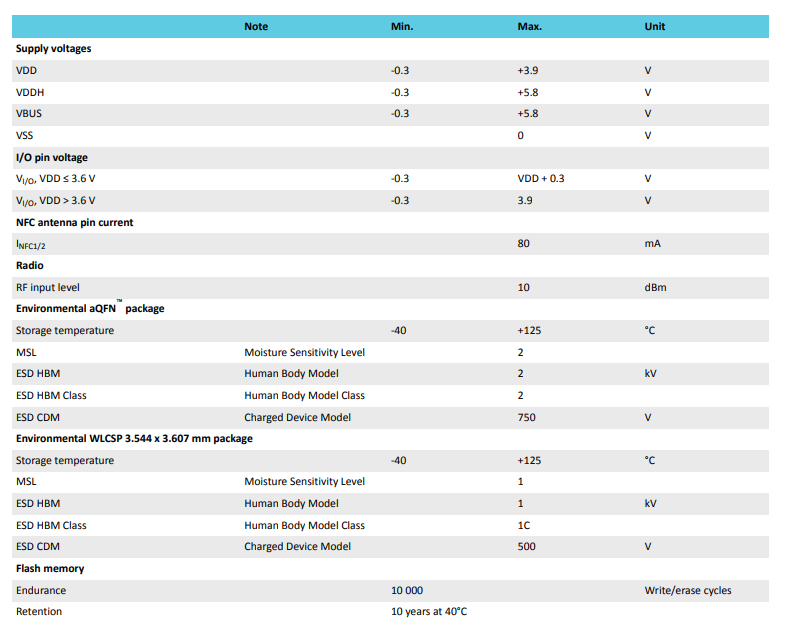
\includegraphics[width=.55\linewidth]{Imagenes/3.png}
 \caption{Características eléctricas de nRF52480. Tomado de \cite{web}.}
 \label{fig3}
 
\end{figure}
\begin{figure}[H]
\centering
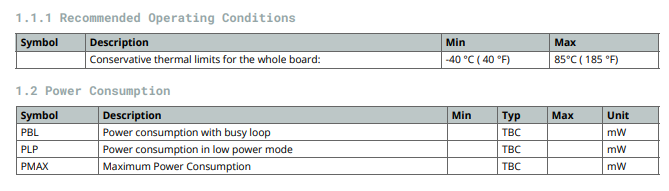
\includegraphics[width=.55\linewidth]{Imagenes/3.1.png}
 \caption{ Características eléctricas de la placa. Tomado de \cite{web2}.}
 \label{fig3.1}
\end{figure}


\subsection*{Periféricos utilizados}
En este laboratorio no se utilizaron periféricos externos, además, el único sensor que se utilizó es el giroscopio de 9 ejes que viene incorporado en el Arduino Nano 33 BLE. A continuación se presentan los puntos más importantes de este sensor (LSM9DS1) para realizar este laboratorio \cite{giroscopio}:
\begin{itemize}
    \item 3 canales de aceleración, 3 canales de velocidad angular, 3 canales de campo magnético.
    \item ±2/±4/±8/±16 g aceleración lineal escala completa.
    \item ±245/±500/±2000 dps velocidad angular escala completa.
    \item Salida de datos de 16 bits.
    \item Interfaces serie SPI / I2C.
    \item Tensión de alimentación analógica 1,9 V a 3,6 V.
\end{itemize}

\begin{figure}[H]
    \centering
    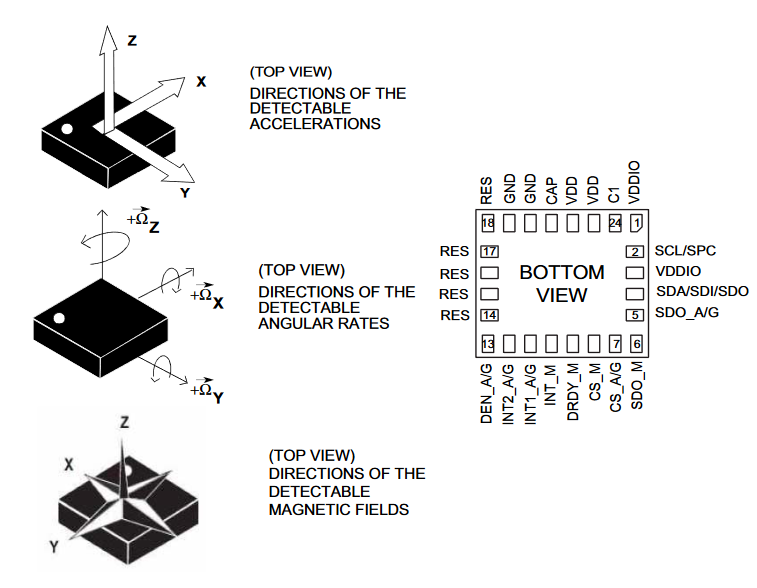
\includegraphics[width=.55\linewidth]{Imagenes/k1.png}
    \caption{Diagrama de pines del LSM9DS1, tomado de \cite{giroscopio}.}
    \label{k1}
\end{figure}


\subsection*{Lista de componentes}
\begin{table}[H]
\caption{Lista de equipos}
\label{table_2}
\begin{center}
\begin{tabular}{r|cc}
\hline
\textbf{Componente}&\textbf{Cantidad}&\textbf{Precio}\\
 \hline
Arduino Nano 33 BLE & 1 & 60\$ \\ \hline 

 \textbf{Total}& & 60\$ \\
 \hline
\end{tabular}
\end{center}
\end{table}

\subsection*{Diseño del circuito}
El diseño del circuito es muy simple ya que basta con conectar el arduino nano 33 ble sense a la computadora por medio de un cable USB, tal como se muestra en la figura \ref{fig4}.
\begin{figure}[H]
\centering


\tikzset{every picture/.style={line width=0.75pt}} %set default line width to 0.75pt        

\begin{tikzpicture}[x=0.75pt,y=0.75pt,yscale=-1,xscale=1]
%uncomment if require: \path (0,528); %set diagram left start at 0, and has height of 528

%Shape: Rectangle [id:dp7327399467778912] 
\draw   (233,206) -- (233,294) -- (204,294) -- (204,206) -- cycle ;
%Rounded Rect [id:dp2315563507614331] 
\draw   (307,153.2) .. controls (307,145.91) and (312.91,140) .. (320.2,140) -- (384.8,140) .. controls (392.09,140) and (398,145.91) .. (398,153.2) -- (398,192.8) .. controls (398,200.09) and (392.09,206) .. (384.8,206) -- (320.2,206) .. controls (312.91,206) and (307,200.09) .. (307,192.8) -- cycle ;
%Curve Lines [id:da34814740280768275] 
\draw    (234,247) .. controls (298.35,242.05) and (224.51,162.61) .. (303.56,172.67) ;
\draw [shift={(306,173)}, rotate = 188.23] [fill={rgb, 255:red, 0; green, 0; blue, 0 }  ][line width=0.08]  [draw opacity=0] (8.93,-4.29) -- (0,0) -- (8.93,4.29) -- cycle    ;

% Text Node
\draw (342,164) node [anchor=north west][inner sep=0.75pt]   [align=left] {PC};
% Text Node
\draw (227,211) node [anchor=north west][inner sep=0.75pt]  [rotate=-90] [align=left] {{\scriptsize arduino 33 BLE}};
\end{tikzpicture}
\caption{ Diagrama del circuito.}
\label{fig4}
\end{figure}
A partir de lo mostrado anteriormente se consultaron las referencias dadas por el profesor para realizar el laboratorio.
\newpage

\section{Desarrollo/Análisis}
Gracias a lo consultado en \cite{web3}, fue posible realizar todas las configuraciones necesarias para empezar con el uso del programa \texttt{IMU\_ Capture.ino} disponible en \cite{ArduinoSketches1}, el cual se encarga de leer la aceleración y el giroscopio de la placa e imprime por un segundo en el monitor serial (por consola del IDE) cuando una velocidad significativa es detectada. Además, es posible activar el \texttt{Serial Plotter} para graficar los datos. Lo anterior se muestra a continuación.

\begin{figure}[H]
   \begin{minipage}{0.48\textwidth}
     \centering
     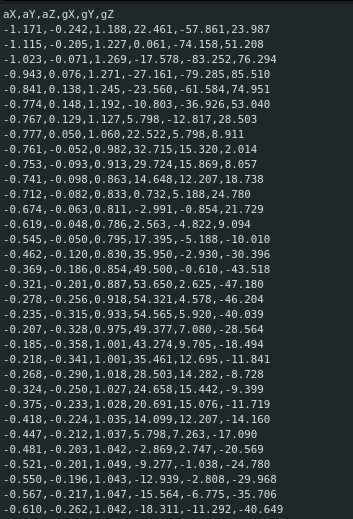
\includegraphics[width=.7\linewidth]{Imagenes/4}
     \caption{ Registro del giroscopio}\label{Fig_4}
   \end{minipage}\hfill
   \begin{minipage}{0.7\textwidth}
     \centering
     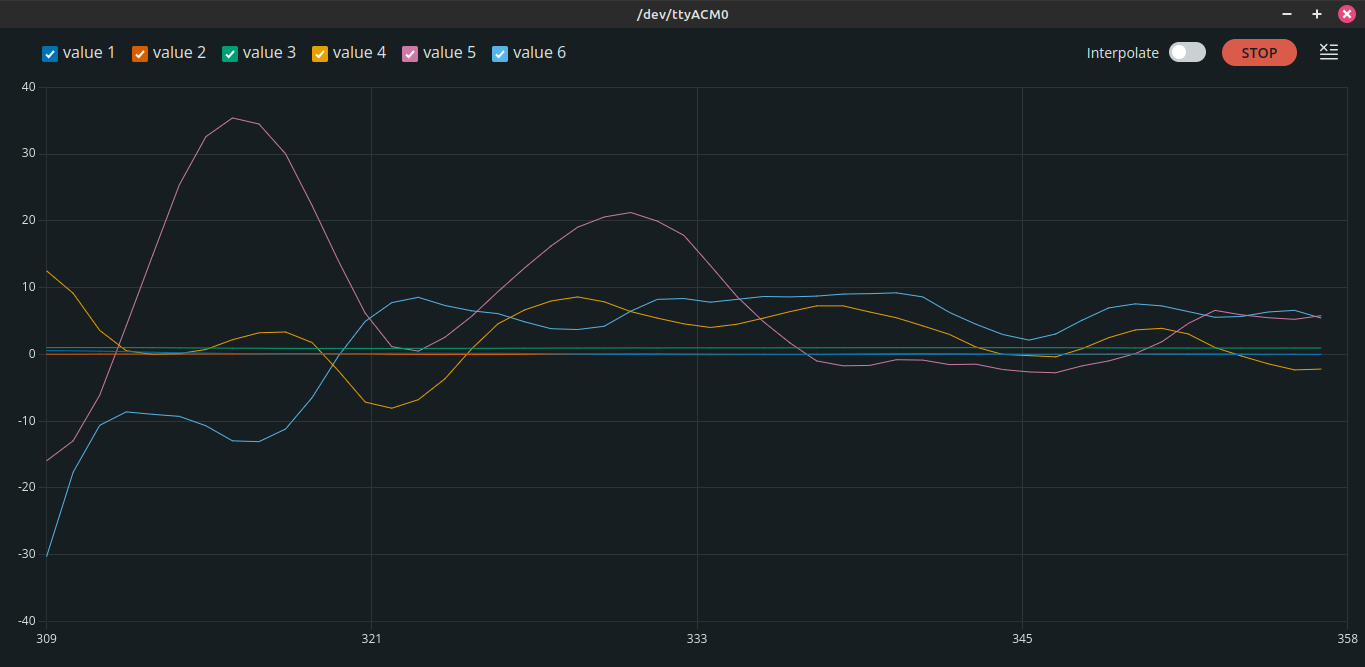
\includegraphics[width=.7\linewidth]{Imagenes/5.png}
     \caption{Graficación del movimiento }\label{Fig_5}
   \end{minipage}
\end{figure}
De la figura \ref{Fig_4}, se tiene las coordenadas que registran el movimiento realizado, que de hecho es un golpe hacia la pantalla de la PC. Luego, en la figura \ref{Fig_5} muestra las ondas del golpe. Hecho esto, se procede a realizar un pequeño script de Python para grabar todos estos datos en un archivo .csv. Por lo que una vez cargado el código \texttt{IMU\_ Capture.ino} se cierra el IDE de Arduino y se ejecuta el script. De donde se realizaron 3 movimientos.
\begin{itemize}
\item Golpe hacia la pantalla (en una sola dirección).
\item Alzar el brazo con diferentes direcciones.
 \item Movimiento circular en contra de las manecillas del reloj.
\end{itemize}
Se tomaron 1750 muestras para los 3 movimientos, un aproximado de \SI{25}{\s} realizando la misma tarea. Ahora, con base a estos datos se realizó el entrenamiento con ayuda de \cite{web4}.\par

%\begin{figure}[H]
%\centering
%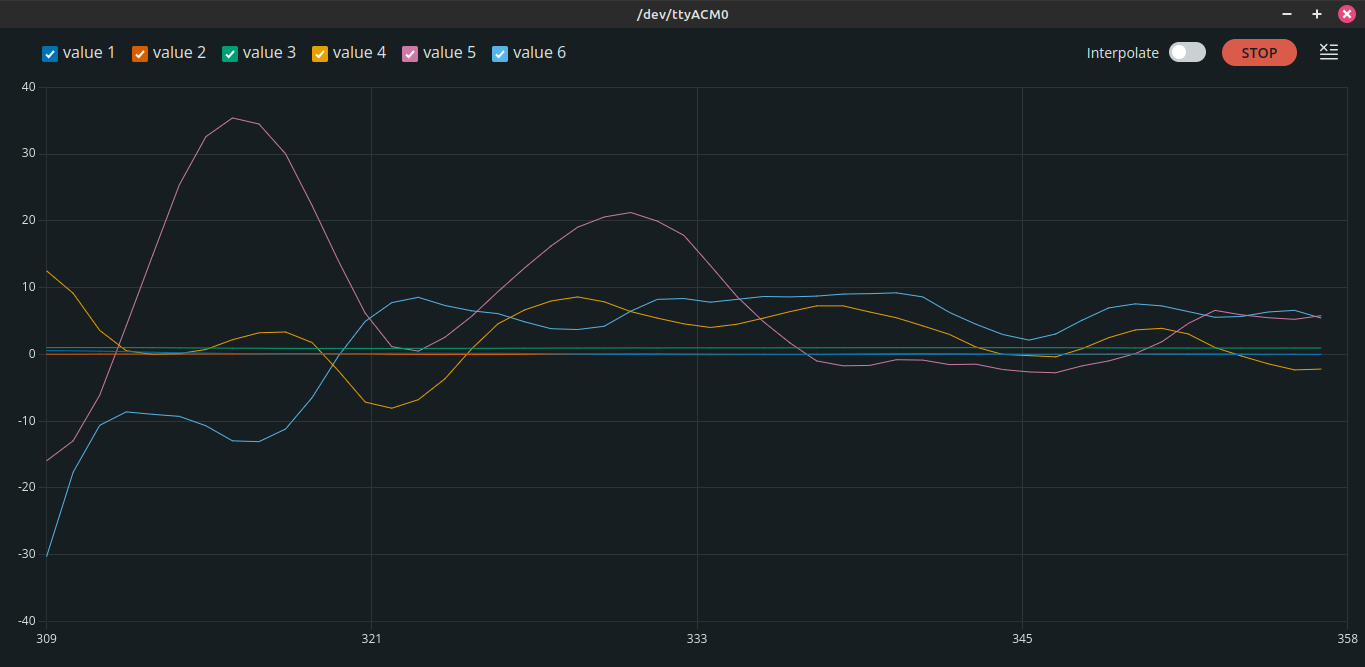
\includegraphics[width=.55\linewidth]{Imagenes/5.png}
% \caption{Funcionamiento del giroscopio.}
% \label{fig_gyro}
%\end{figure}

Para el entrenamiento se tomaron los resultados obtenidos y se procedió a usar como base el ejemplo de reconocimiento de gestos dado en la presentación de la clase \cite{web4}.
El primer paso fue introducir los datos, el resultado de esto se observa a continuación:
\begin{figure}[H]
    \centering
    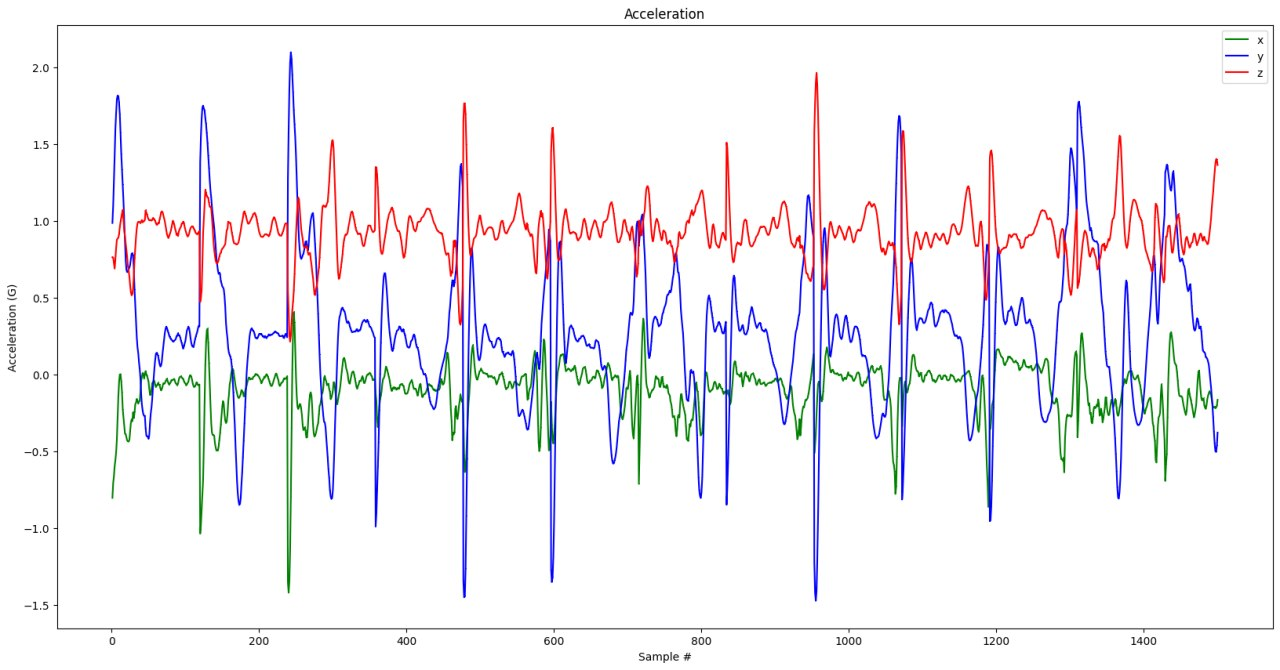
\includegraphics[width=.65\linewidth]{Imagenes/k (1).jpg}
    \caption{Datos de aceleración importados.}
\end{figure}

\begin{figure}[H]
    \centering
    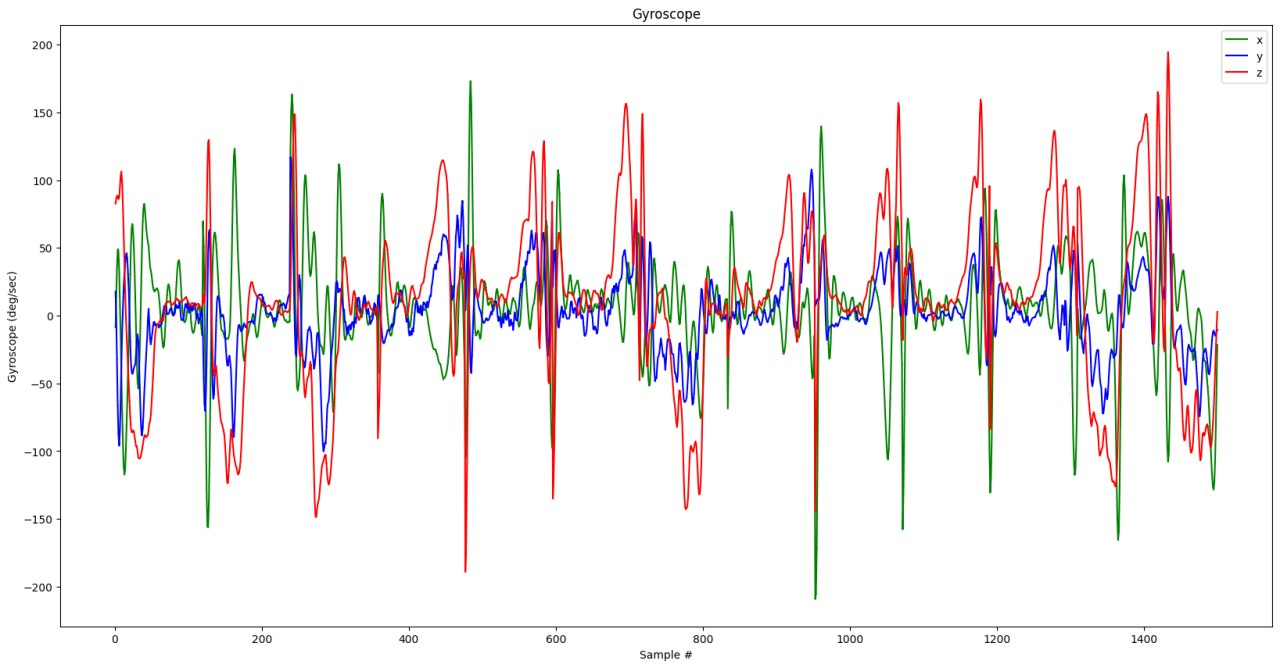
\includegraphics[width=.65\linewidth]{Imagenes/k (2).jpg}
    \caption{Datos del giroscopio importado.}
\end{figure}

Una vez realizado este paso se empieza a entrenar el modelo, para ello se preparan los datos para que su formato coincida, una vez realizado lo anterior se entrena la red siguiendo las indicaciones del enunciado y tomando el 60\% de los datos para el entrenamiento, un 20\% para la validación y otro 20\% para realizar pruebas. Los resultados del entrenamiento se muestran en las siguientes figuras:
\begin{figure}[H]
    \centering
    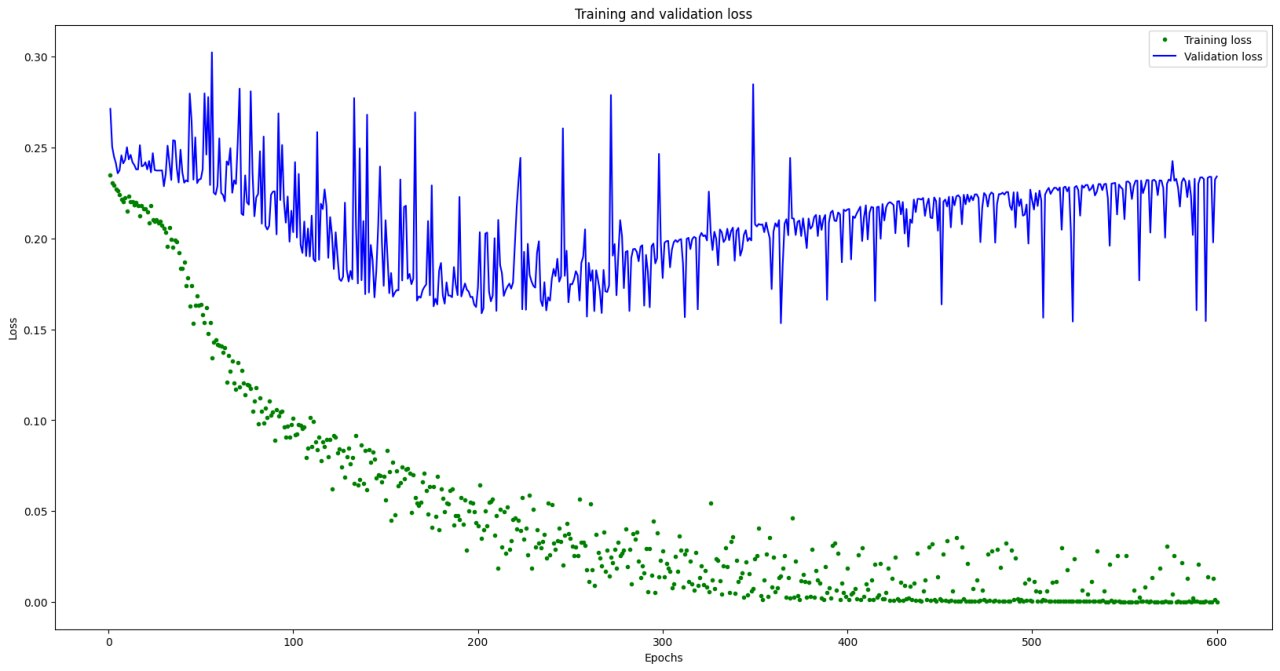
\includegraphics[width=.65\linewidth]{Imagenes/k (3).jpg}
    \caption{Gráfica del entrenamiento y su pérdida.}
\end{figure}

\begin{figure}[H]
    \centering
    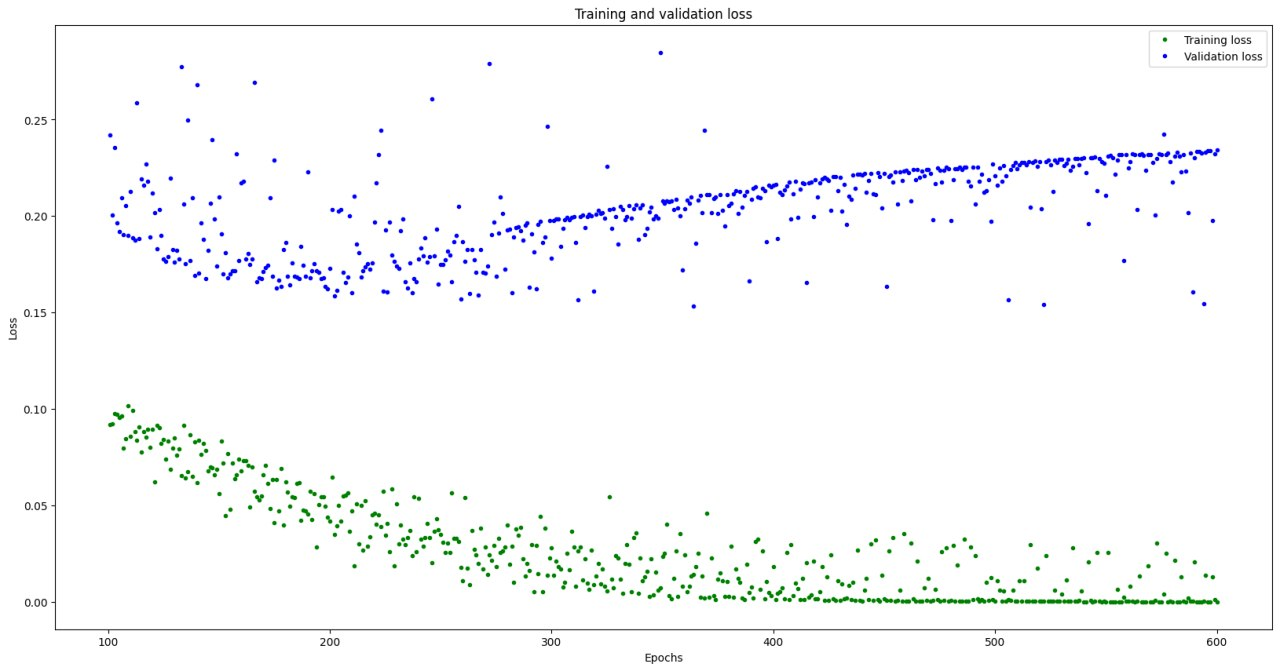
\includegraphics[width=.65\linewidth]{Imagenes/k (4).jpg}
    \caption{Gráfica del entrenamiento y su pérdida iniciando en 100.}
\end{figure}

\begin{figure}[H]
    \centering
    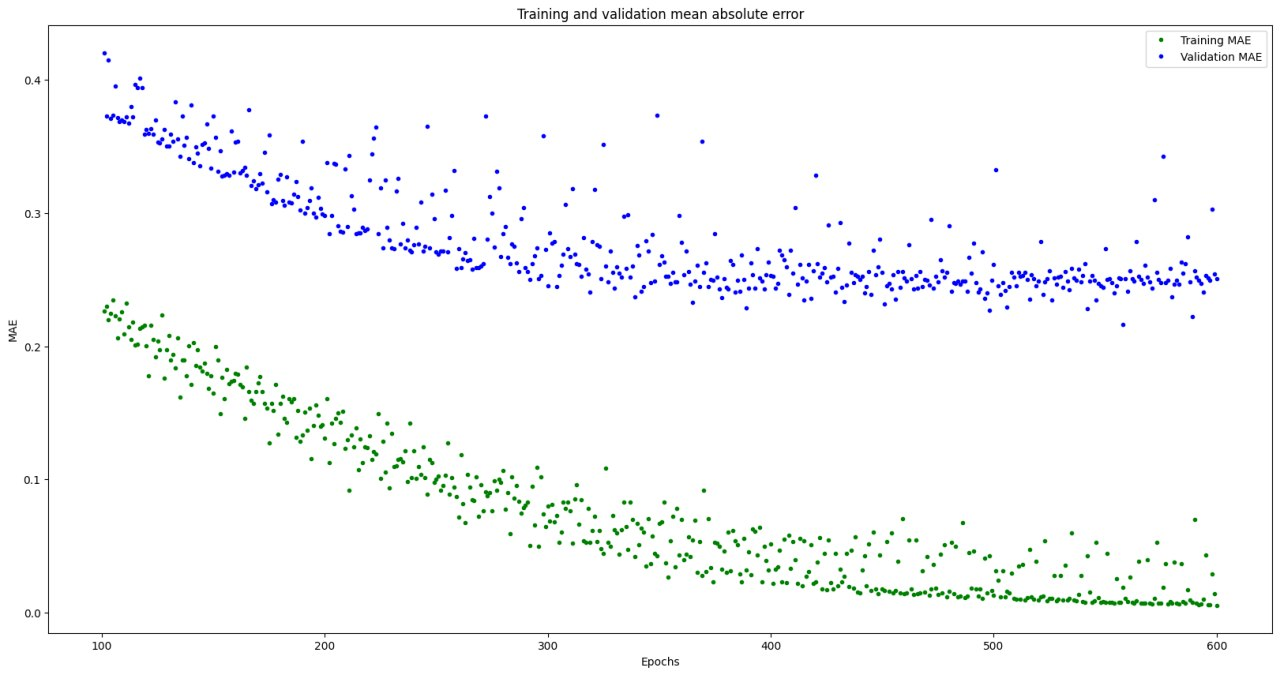
\includegraphics[width=.65\linewidth]{Imagenes/k (5).jpg}
    \caption{Gráfica del error absoluto para observar rendimiento.}
\end{figure}

Con lo anterior se obtiene un archivo de encabezado ''model.h'' que es usado para poder determinar los movimientos escogidos para este laboratorio.\\

Ahora, gracias al entrenamiento realizado y siguiendo con la ayuda de los ejemplos vistos en clase, se toma la referencia de \cite{ArduinoSketches1} a la cual se le hacen unas pequeñas modificaciones, primero se le añade el archivo \texttt{model.h} para ver los resultados del entramiento pero ahora en la placa.
Lo otro es la eliminación de algunos encabezados que no serán necesarios ya que el profesor indicó que son más orientados a los desarrolladores de tensorflow tales como: \texttt{tensorflow/lite/micro/micro\_error\_ reporter.h} y \texttt{tensorflow/lite/version.h}. También se eliminó la variable global \texttt{tflite::MicroErrorReporter tflErrorReporter} y el acceso a la memoria de esta misma variable. Por otro, lado se tuvo que añadir los mapas de los gestos:\newpage
\begin{lstlisting}[label={mini_bloque}, caption={Nombre de los archivos csv}]
// array to map gesture index to a name
const char* GESTURES[] = {
  "punch",
  "arm_up",
  "circle"
};
\end{lstlisting}

Hecho esto, se verificó y cargó el código a la placa, lo cual tomó cierto tiempo en comparación a otros ejemplos. Una vez terminado esto, se realizaron los movimientos y por medio del serial monitor se mostraron las probabilidades de los movimientos ejecutados, donde el que posee mayor probabilidad indica  el movimiento o acción hecha con la placa.
\begin{figure}[H]
   \begin{minipage}{0.5\textwidth}
     \centering
     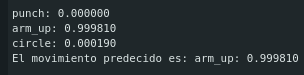
\includegraphics[width=.48\linewidth]{Imagenes/arm_up.png}
     \caption{ Movimiento brazo arriba.}\label{arm_up}
   \end{minipage}\hfill
   \begin{minipage}{0.5\textwidth}
     \centering
     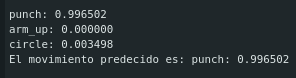
\includegraphics[width=.48\linewidth]{Imagenes/punch.png}
     \caption{Movimiento puño hacia la PC. }\label{punch}
   \end{minipage}
      \begin{minipage}{0.5\textwidth}
     \centering
     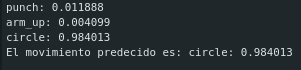
\includegraphics[width=.48\linewidth]{Imagenes/circle.png}
     \caption{Movimiento circular. }\label{circle}
   \end{minipage}
    \begin{minipage}{0.5\textwidth}
     \centering
     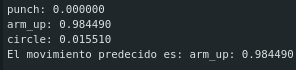
\includegraphics[width=.48\linewidth]{Imagenes/brazo_up.png}
     \caption{Movimiento brazo arriba. }\label{brazo_up}
   \end{minipage}
\end{figure}
Primero se levantó el brazo y es sencillo notar que en la figura \ref{arm_up} el movimiento es detectado correctamente ya que las demás probabilidades o valores con base al entrenamiento fueron totalmente despreciables. El siguiente movimiento fue un puñetazo hacia la PC y note que en la figura \ref{punch} la placa logra detectarlo sin problema alguno, con una similitud muy ínfima con el movimiento circular. Por último, se movió la placa en forma circular y el resultado de la figura \ref{circle} detecta este movimiento con algunas similitudes con el levantamiento del brazo hacia y el puñetazo, no obstante el valor más alto fue el movimiento circular. En resumen, la figura \ref{moves} es la consola o el monitor serial de Arduino que va mostrando estas probabilidades dependiendo del movimiento que se ejecute con la placa.
\begin{figure}[H]
\centering
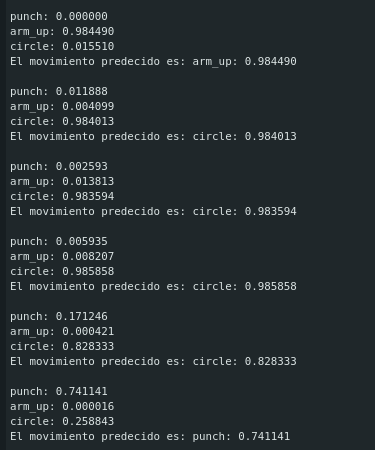
\includegraphics[width=.40\linewidth]{Imagenes/11.png}
 \caption{Resumen de los movimientos.}
 \label{moves}
\end{figure}

\newpage


\newpage
\section{Conclusiones y recomendaciones}
Las conclusiones para este trabajo son:
\begin{itemize}
\item Los ejemplos brindados fueron de gran ayuda para realizar las pruebas con el giroscopio.
\item El notebook de Colab está muy bien hecho porque es rápido, lo cual tiene sentido al tratarse de Python, y realiza un muy buen entrenamiento de los datos porque a la hora de llevar el archivo \texttt{model.h} al código \texttt{IMU\_ Classifier}, resulta que que la placa es consistente cuando asigna una probabilidad al movimiento realizado previamente.
\item Tensorflow lite es una herramienta muy poderosa porque permite hacer uso de técnicas de machine learning en dispositivos que no tienen un rendimiento tan alto.
\item Por tanto, el programa cumple satisfactoriamente porque los movimientos realizados fueron hechos con la misma cantidad de muestras; 1750. Para el caso del puñetazo se hizo en una misma dirección hacia la pantalla de la PC. En cambio, los otros dos: movimiento circular se ejecutó en sentido horario y anti-horario, y el brazo hacia arriba se hizo en diferentes ejes. Además, el buen entrenamiento de los datos mencionado previamente ayudó mucho para identificar los movimientos realizados.
\end{itemize}
A modo de recomendación, prestar mucha atención en clases con \textbf{todo} lo que menciona el profesor, por supuesto estudiar muy bien los ejemplos recomendados por él así como la literatura. Lo otro muy importante es hacer los movimientos con diferentes ejes y así no tener un mismo patrón en un muestreo de 1750 muestras ya que no habrá diversidad para identificar el movimiento realizado.


\newpage 

\bibliographystyle{unsrt}
\bibliography{bibliografia.bib}
\newpage

  \section{Anexos}
 A continuación, se muestran las hojas del fabricante de los componentes usados para este laboratorio. Y el link del repositorio de este trabajo: \url{https://github.com/JosueC07183/Labo5}.

%\includepdf[pages=1-14]{./Documentos/A000066-datasheet.pdf}
\foreach \page in {2,3,18}{
  \includepdf[pages=\page]{./Documentos/nRF52840_PS_v1.1.pdf}
}
\foreach \page in {1, 2,3, 10}{
  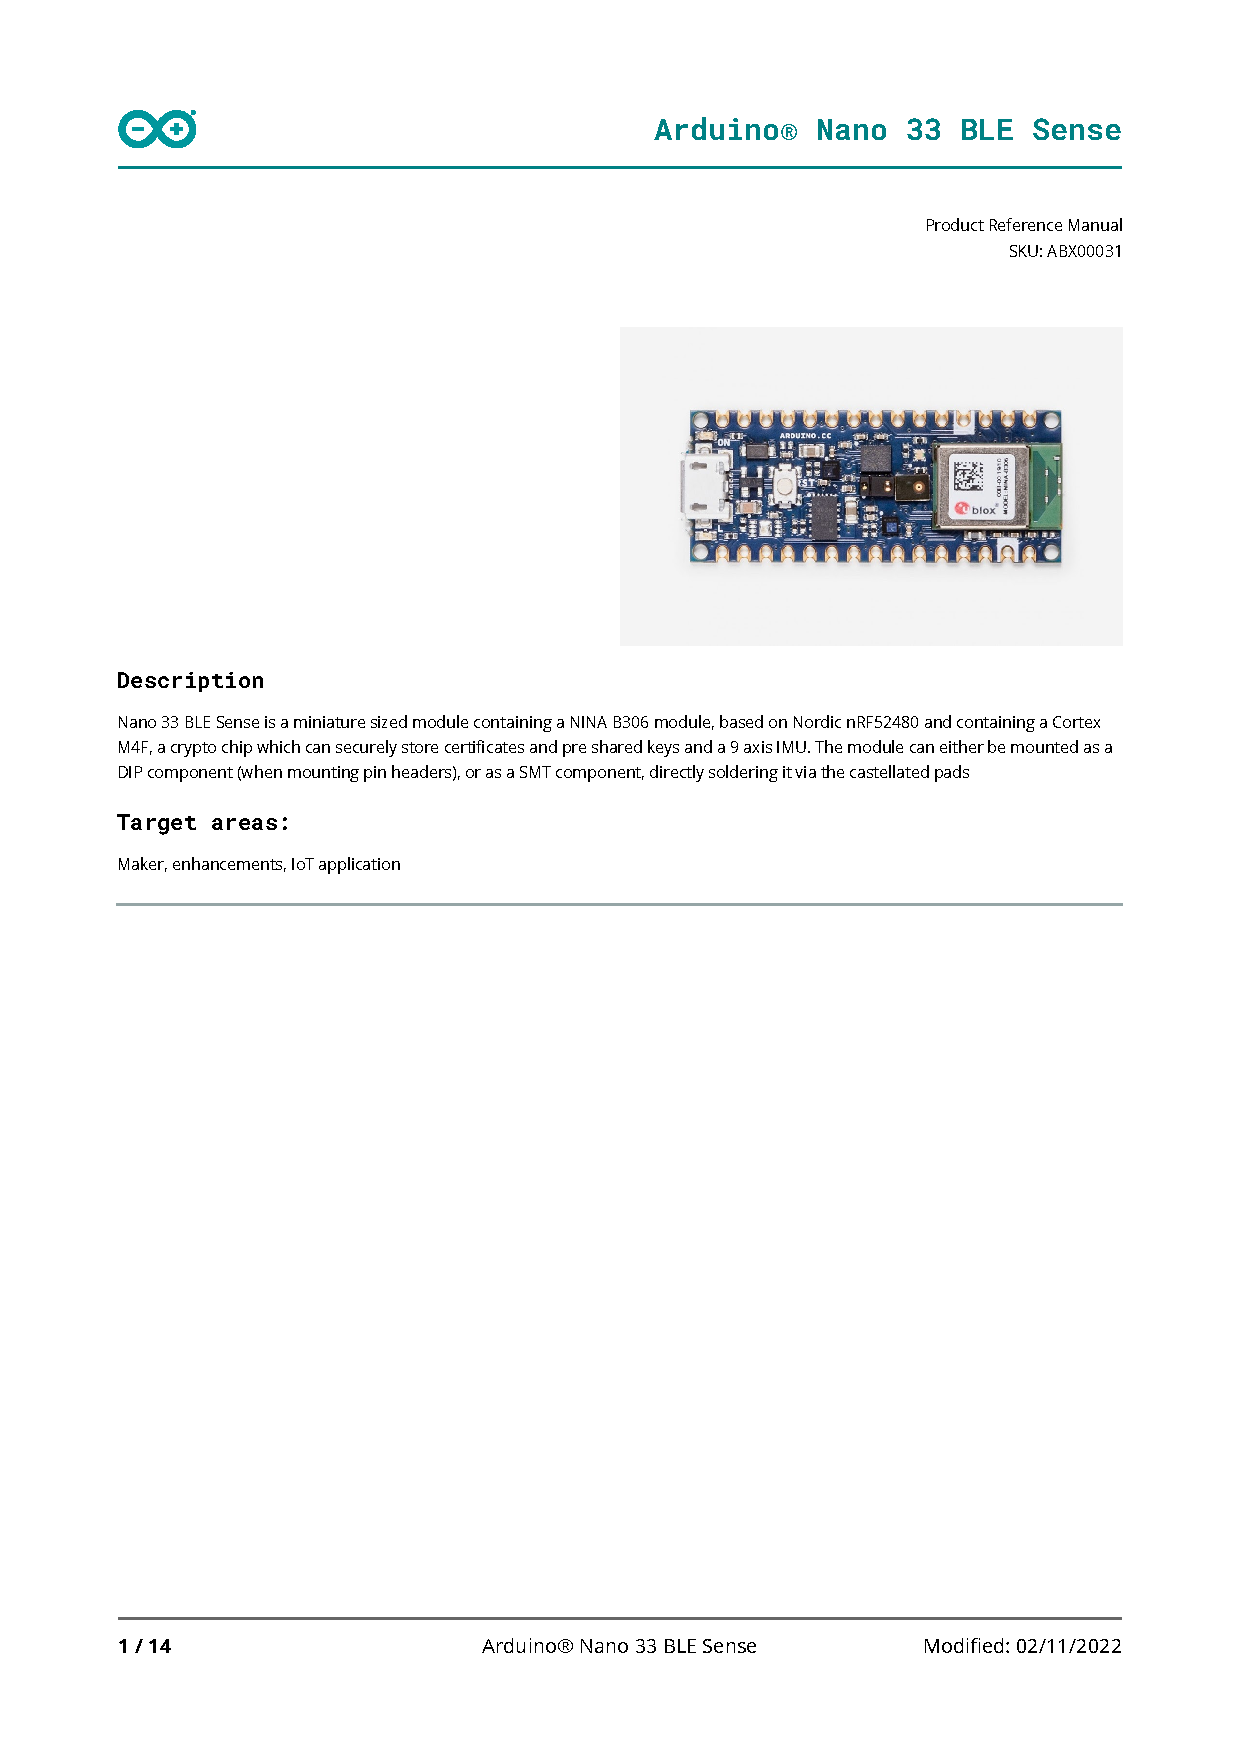
\includepdf[pages=\page]{./Documentos/DatasheetNano33BLE.pdf}
}

\end{document}
 

\end{document}